\documentclass[10pt,a4paper,landscape]{article}
\usepackage[margin=1.15cm]{geometry}
\usepackage{graphicx}
\graphicspath{{assets/}{../../assets/}}
\usepackage{array,tabularx}
\usepackage{amsmath}
\usepackage{tikz}
\usepackage{xcolor}
\usepackage{enumitem}
\usepackage{fancyhdr}
\usepackage{lastpage}
\setlength{\parindent}{0pt}
\setlength{\parskip}{3pt}
\renewcommand{\arraystretch}{1.35}
\pagestyle{fancy}
\fancyhf{}
\lfoot{Instituto Jorge Robledo · Foundations of Physics 9th}
\rfoot{Page \thepage\ of \pageref{LastPage}}
\renewcommand{\headrulewidth}{0pt}
\renewcommand{\footrulewidth}{0.3pt}
\newcommand{\blank}[1]{\rule{#1}{0.4pt}}
\newcommand{\ijrlogo}[1]{\IfFileExists{assets/logo_colegio_fondo_blanco.png}{\includegraphics[width=#1]{assets/logo_colegio_fondo_blanco.png}}{\IfFileExists{../../assets/logo_colegio_fondo_blanco.png}{\includegraphics[width=#1]{../../assets/logo_colegio_fondo_blanco.png}}{}}}

\begin{document}

\begin{minipage}[c]{0.08\textwidth}
\ijrlogo{1.55cm}
\end{minipage}
\begin{minipage}[c]{0.90\textwidth}
{\Large\bfseries Galileo Inclined Plane — 1 Hour Laboratory}\\[-1mm]
{\small Grade 9 · Group work: 3 students per table · Student data sheet}
\end{minipage}

\vspace{2mm}\hrule\vspace{2mm}

\begin{tabularx}{\textwidth}{@{}X X X X@{}}
\textbf{Student 1:} \blank{4.3cm} & \textbf{Student 2:} \blank{4.3cm} & \textbf{Student 3:} \blank{4.3cm} & \textbf{Section / Date:} \blank{3.6cm} \\
\end{tabularx}

\vspace{2mm}
\begin{minipage}[t]{0.49\textwidth}
\textbf{Goal.} Test how position depends on time and compare the motion for three different inclinations of the same plane.

\textbf{Keep the same in every configuration:} same object, same start line, same four position marks, and same measuring method.

\textbf{Roles — rotate after each configuration:}
\begin{itemize}[leftmargin=5mm,itemsep=0pt,topsep=1pt]
  \item Student A: releases the object without pushing it.
  \item Student B: measures time (tablet/video or stopwatch).
  \item Student C: records data and checks units.
\end{itemize}
\end{minipage}
\hfill
\begin{minipage}[t]{0.49\textwidth}
\textbf{60-minute plan}
\begin{tabular}{@{}ll@{}}
0--10 min & Set up ramp, choose four marks, make one test run.\\
10--35 min & Measure Low, Medium, and High inclination.\\
35--50 min & Calculate $\bar t$ and $\bar t^{\,2}$; make the graph.\\
50--60 min & Answer the four conclusion questions.\\
\end{tabular}

\textbf{Procedure}
\begin{enumerate}[leftmargin=5mm,itemsep=0pt,topsep=1pt]
  \item Mark the start as $x=0$. Choose four positions along the usable ramp.
  \item For each position, measure the travel time twice and calculate the mean time $\bar t$.
  \item Calculate $\bar t^{\,2}$.
  \item Repeat for three plane inclinations: Low, Medium, High.
  \item Plot all three data sets on the same graph: $x$ versus $t^2$.
\end{enumerate}
\end{minipage}

\vspace{2mm}\hrule\vspace{2mm}

\newcommand{\datatable}[1]{%
\begin{minipage}[t]{0.325\textwidth}
\centering
{\bfseries #1}\\[-1mm]
{\small Rise $h=$ \blank{1.7cm} cm \quad Angle $\theta=$ \blank{1.4cm}$^\circ$ \; (if available)}\\[1mm]
\begin{tabular}{|>{\centering\arraybackslash}p{1.15cm}|>{\centering\arraybackslash}p{1.25cm}|>{\centering\arraybackslash}p{1.25cm}|>{\centering\arraybackslash}p{1.35cm}|>{\centering\arraybackslash}p{1.50cm}|}
\hline
\textbf{$x$ (m)} & \textbf{$t_1$ (s)} & \textbf{$t_2$ (s)} & \textbf{$\bar t$ (s)} & \textbf{$\bar t^2$ (s$^2$)} \\
\hline
 & & & & \\
\hline
 & & & & \\
\hline
 & & & & \\
\hline
 & & & & \\
\hline
\end{tabular}
\end{minipage}}

\datatable{Configuration 1 — LOW}\hfill
\datatable{Configuration 2 — MEDIUM}\hfill
\datatable{Configuration 3 — HIGH}

\vfill
{\small\textbf{Quick check:} all three configurations must use the same four $x$ positions. If one timing is clearly bad, repeat that measurement once.}

\newpage

\begin{minipage}[c]{0.08\textwidth}
\ijrlogo{1.35cm}
\end{minipage}
\begin{minipage}[c]{0.90\textwidth}
{\Large\bfseries Graph and Conclusion}\\[-1mm]
{\small Plot $x$ on the vertical axis and $t^2$ on the horizontal axis. Use a different symbol for each inclination.}
\end{minipage}

\vspace{2mm}\hrule\vspace{2mm}

\begin{center}
\textbf{Legend:} \quad LOW $\circ$ \qquad MEDIUM $\triangle$ \qquad HIGH [ ]
\end{center}

\begin{center}
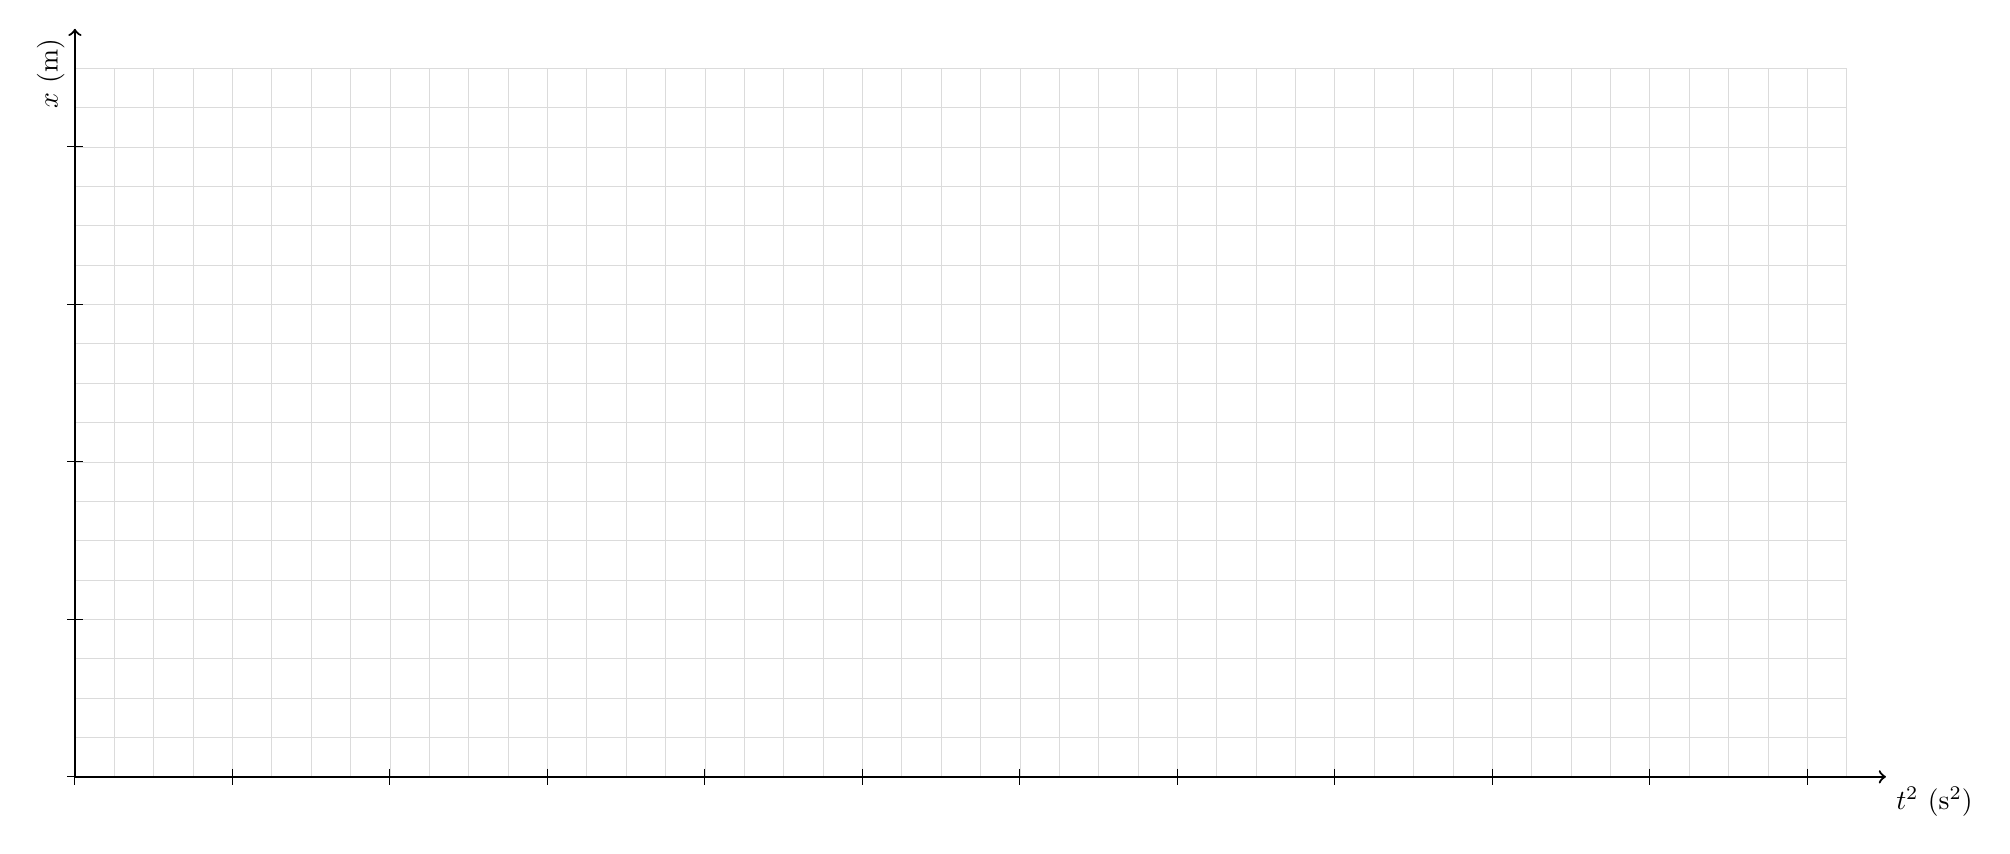
\begin{tikzpicture}[x=1cm,y=1cm]
  \draw[step=0.5cm,gray!28,very thin] (0,0) grid (22.5,9.0);
  \draw[->,thick] (0,0) -- (23.0,0) node[below right] {$t^2$ (s$^2$)};
  \draw[->,thick] (0,0) -- (0,9.5) node[above left,rotate=90] {$x$ (m)};
  \foreach \x in {0,2,4,6,8,10,12,14,16,18,20,22} {\draw (\x,0.10)--(\x,-0.10);}
  \foreach \y in {0,2,4,6,8} {\draw (0.10,\y)--(-0.10,\y);}
\end{tikzpicture}
\end{center}

\vspace{-1mm}
\begin{tabularx}{\textwidth}{@{}X X@{}}
\textbf{1.} Is $x$ versus $t^2$ approximately a straight line? \blank{4.8cm} &
\textbf{2.} Which configuration has the steepest line? \blank{4.5cm} \\
\rule{0pt}{0.9cm}\textbf{Why?} \blank{9.8cm} &
\textbf{What does that mean physically?} \blank{7.2cm} \\
\textbf{3.} As the plane becomes steeper, acceleration: \quad increases / decreases / stays the same. &
\textbf{4.} Complete: for motion starting from rest, our data support $x \propto$ \blank{1.8cm}. \\
\end{tabularx}

\vspace{1mm}\hrule\vspace{1mm}
{\small\textbf{Galileo connection:} a straight $x$ versus $t^2$ graph supports $x\propto t^2$. For release from rest, $x=\tfrac12 at^2$. A steeper line means a larger acceleration.}

\end{document}
